\section{Experiment Results and discussion}
\subsection{Experiments based on Hebbian learning rule}
\subsubsection{Experiments results}

\begin{figure}[h]
\centering
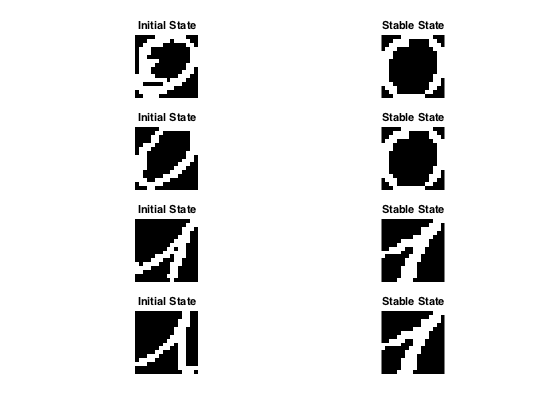
\includegraphics[scale=0.3]{2st.png}
\caption{Experiment result of storing two memories(digits 0 and 1) in network}
\label{fg:ex1}
\end{figure}

We can start with storing two memories(digits 0 and 1) in the Hopfield network first. As shown in the Figure \ref{fg:ex1}, all of test cases are successfully convergence into the correct stable state. \\

\begin{figure}[h]
\centering
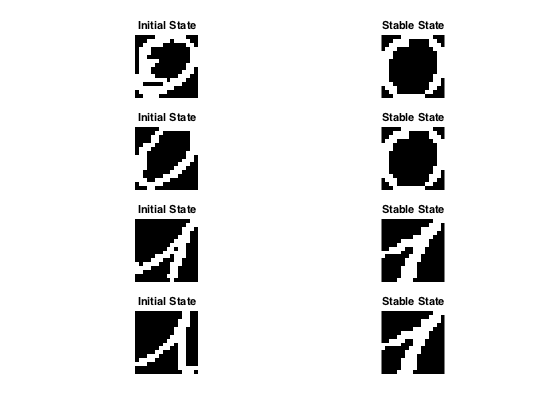
\includegraphics[scale=0.3]{3st.png}
\caption{Experiment result of storing three memories(digits 0, 1 and 2) in network}
\label{fg:ex2}
\end{figure}

In Figure \ref{fg:ex2}, we can notice that, when we store 3 memories(digits 0, 1 and 2), all test cases also could convergence into the correct stable state. \\

\begin{figure}[h]
\centering
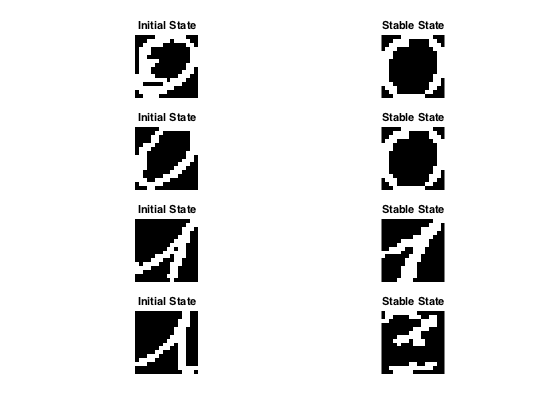
\includegraphics[scale=0.3]{4st.png}
\caption{Experiment result of storing four memories(digits 0, 1, 2 and 4) in network}
\label{fg:ex3}
\end{figure}

As shown in Figure \ref{fg:ex3}, When 4 memories(digits 0, 1, 2 and 3) stores in the Hopfield network, the first three samples still could convergence to the correct stable state. However, the fourth sample digit 1 converge into a spurious stable state which likes a mixture state of digit 2 and 3. it is possible that this mixture state could have a lower energy compare with sample digit 1 that we stored in Hopfield network. \\

\begin{figure}[h]
\centering
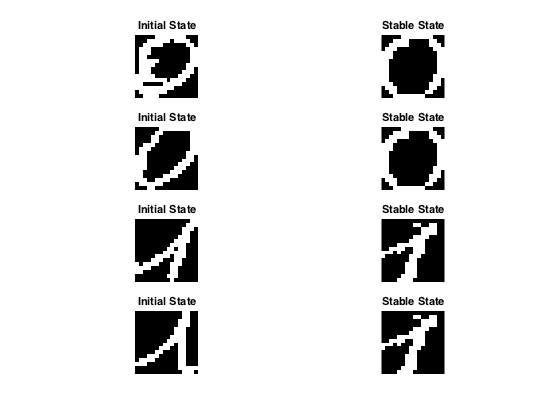
\includegraphics[scale=0.3]{5st.png}
\caption{Experiment result of storing five memories(digits 0, 1, 2, 4 and 5) in network}
\label{fg:ex4}
\end{figure}

We can squash more memories into the network. Figure \ref{fg:ex4} shows a set of five memories(digits 0, 1, 2, 3, 4) storing in the network. We can notice that the first two digit 0 samples could still convergence to the correct stable state. However, two of those digit 1 sample fail to convergence to the correct stable state. Instead of converging to the sample digit 1 we stored in the network, they both converge into the same spurious stable state which is similar with sample digit 1 but have few pixels flipped around the top.\\

\begin{figure}[h]
\centering
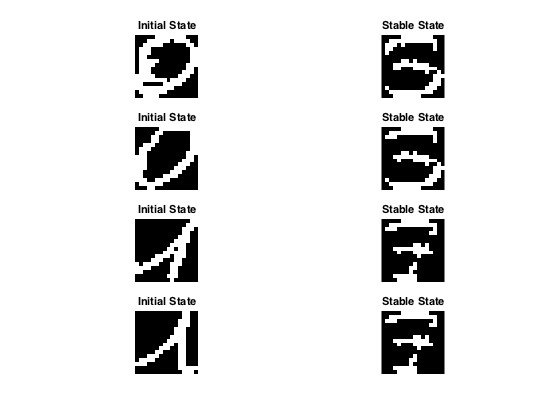
\includegraphics[scale=0.3]{10st.png}
\caption{Experiment result of storing ten memories in network}
\label{fg:ex5}
\end{figure}

In figure \ref{fg:ex5}, We continued add memories into the network up to ten, it can be seen that none of the test cases could converge to one of the stored memories. The first two digit 0 converge to same mixed stable state and the two digit 1 converge converge to a different mixed stable state which closely resembles a digit 7. We found the fact that test cases are tend to converge to some mixed stable states, and believe that these particular mixed stable states must be dominant when running our algorithm with this data set. They are most likely two of the lowest energy states in the entire network.\newpage

\subsubsection{Discussion about experiment results}
\begin{figure}[h]
\centering
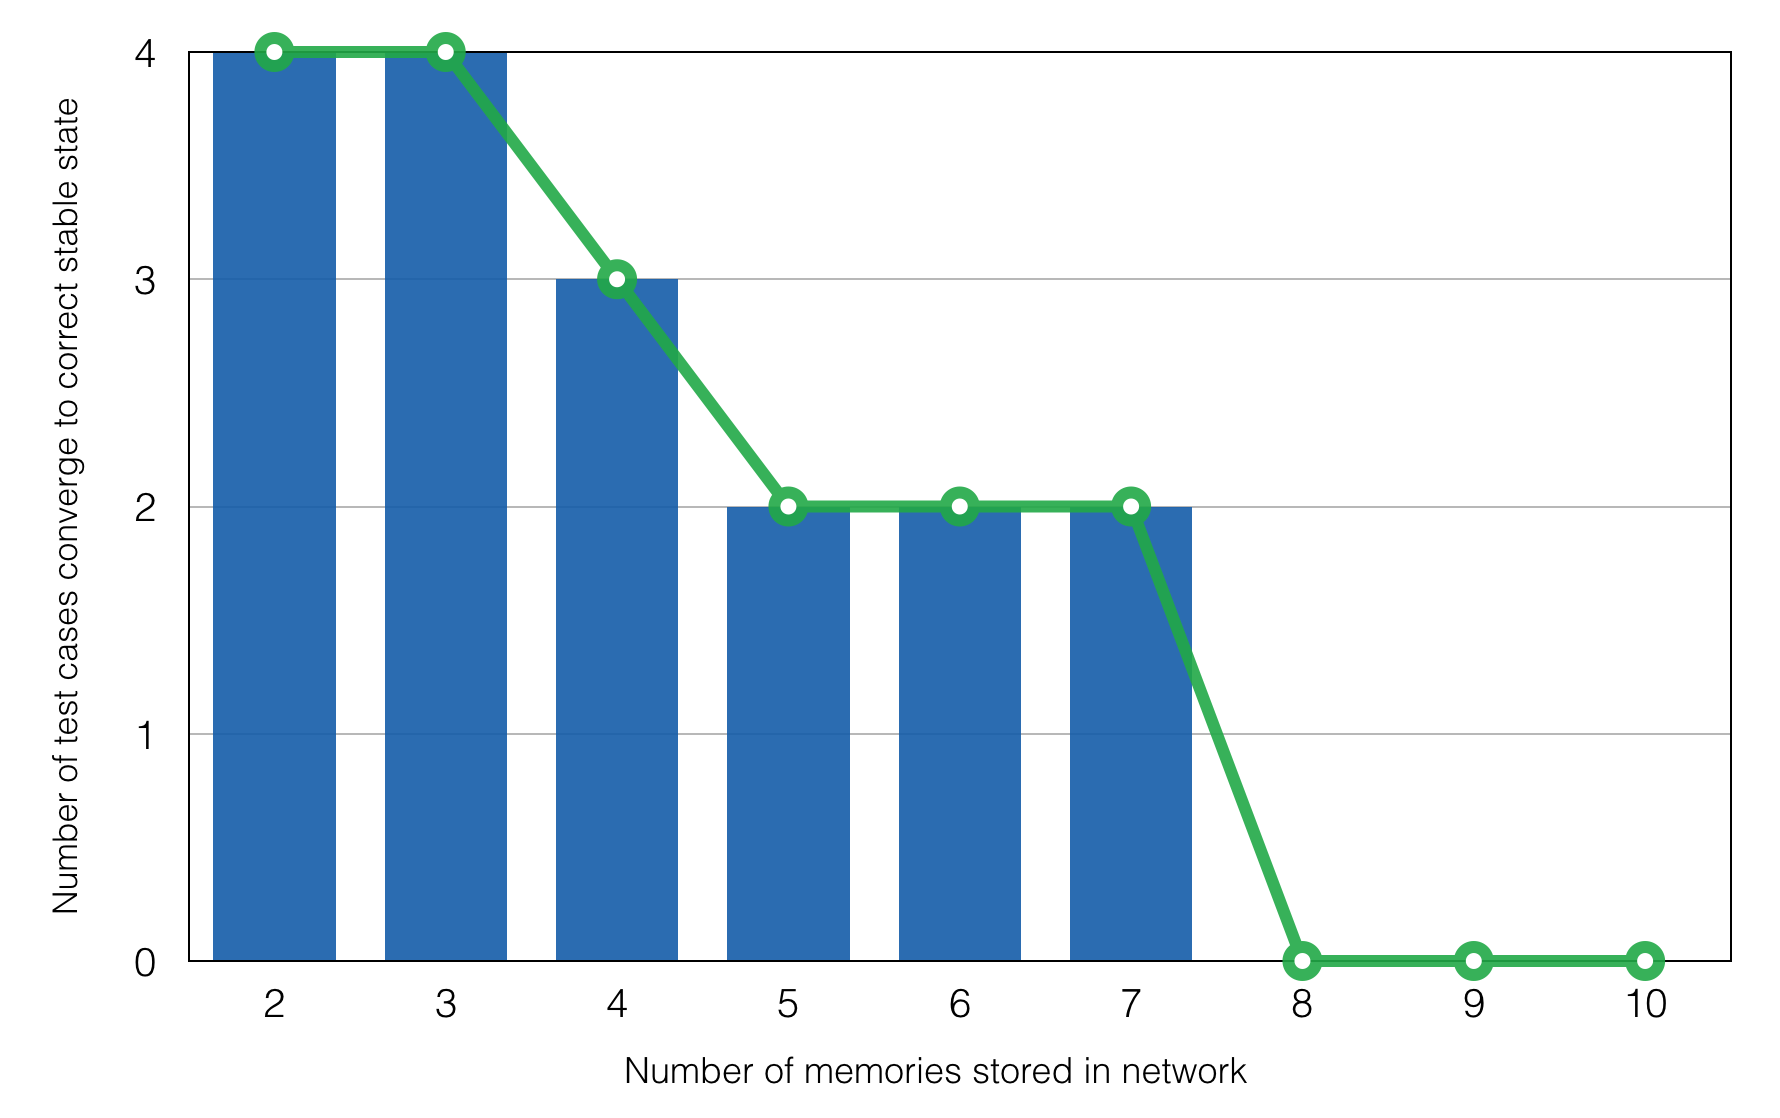
\includegraphics[scale=0.3]{statics1.png}
\caption{the number of test cases that converge to the correct stored memory decreases following the increasing number of memories stored in network}
\label{fg:ex6}
\end{figure}
After looking at the experiment results above, we saw an interesting trend. As shown in Figure \ref{fg:ex6}, it is obvious that as the number of memories stored increases, the number of samples that converge to the correct stored memory decreases. This trend was expected due to the variation of our data set, and the nature of Hopfield networks in general. \newpage

According to the experiment results, Hopfield network model can fail in various ways:\\

\begin{enumerate}
  \item Individual bits in some memories might be corrupted, that is, a stable state of the Hopfield network is displaced a little from the desired memory.
  \item Entire memories might be absent from the list of attractors of the network; or a stable state might be present but have such a small basin of attraction that it is of no use for pattern completion and error correction.
  \item Spurious additional memories unrelated to the desired memories might be present.
  \item Spurious additional memories derived from the desired memories by operations such as mixing and inversion may also be present.
\end{enumerate}

Meanwhile, we also found that as the number of memories stored increases, the possibility of test cases converging into spurious stable states also increases. The reason behind it is that spurious states are tend to have lower energy than those memories(sample digits) we stored in the network when we stored too much memories in the network.\\ 

\subsection{Experiment based on optimized weights}
In the previous section, We observed that as the number of memories stored increases, the number of samples that converge to the correct stored memory decreases. To better illustrate this trend, I decided to run through the data set and record the percentage of correct convergences when storing two, three, five, nine and ten digits. Also, I will implement the objective function (2.6) to optimize the weights matrix and compare its performance with standard weights matrix based on Hebbian learning rule, in hopes of seeing any kind of improvement when using the optimized weights.\\

\begin{figure}[h]
	\centering
	\subfloat[Subfigure 1 list of figures text][Standard weights]{
		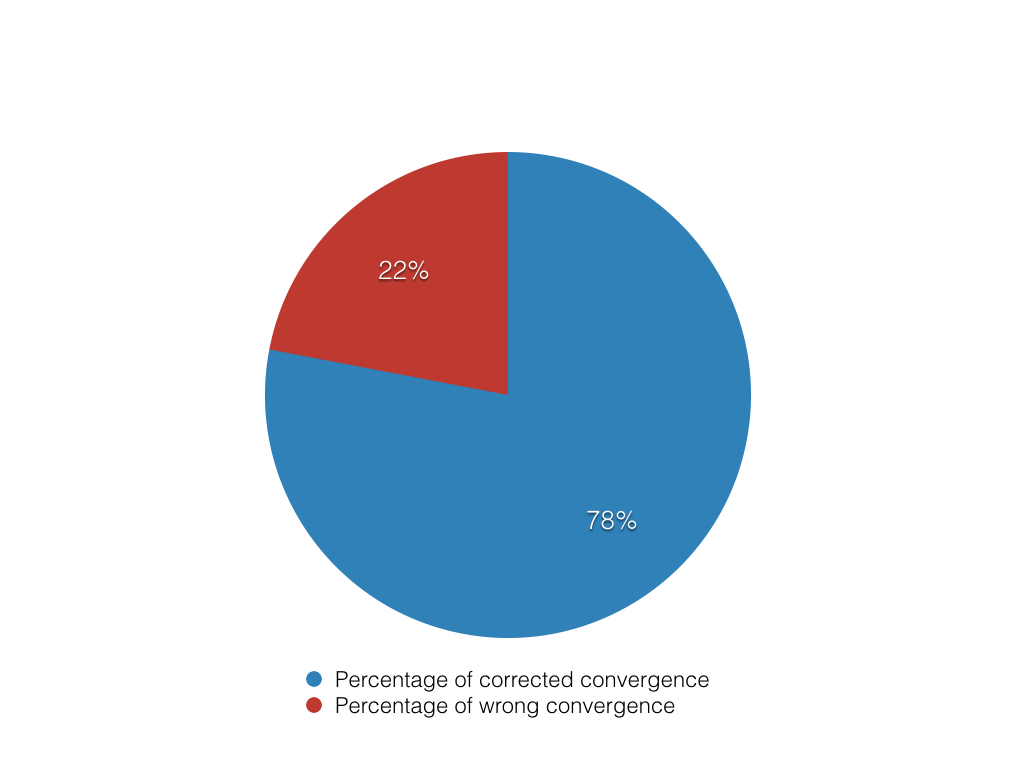
\includegraphics[width=0.5\textwidth]{s2}
		\label{fig:ost11}}
	\subfloat[Subfigure 2 list of figures text][Optimized weights]{
		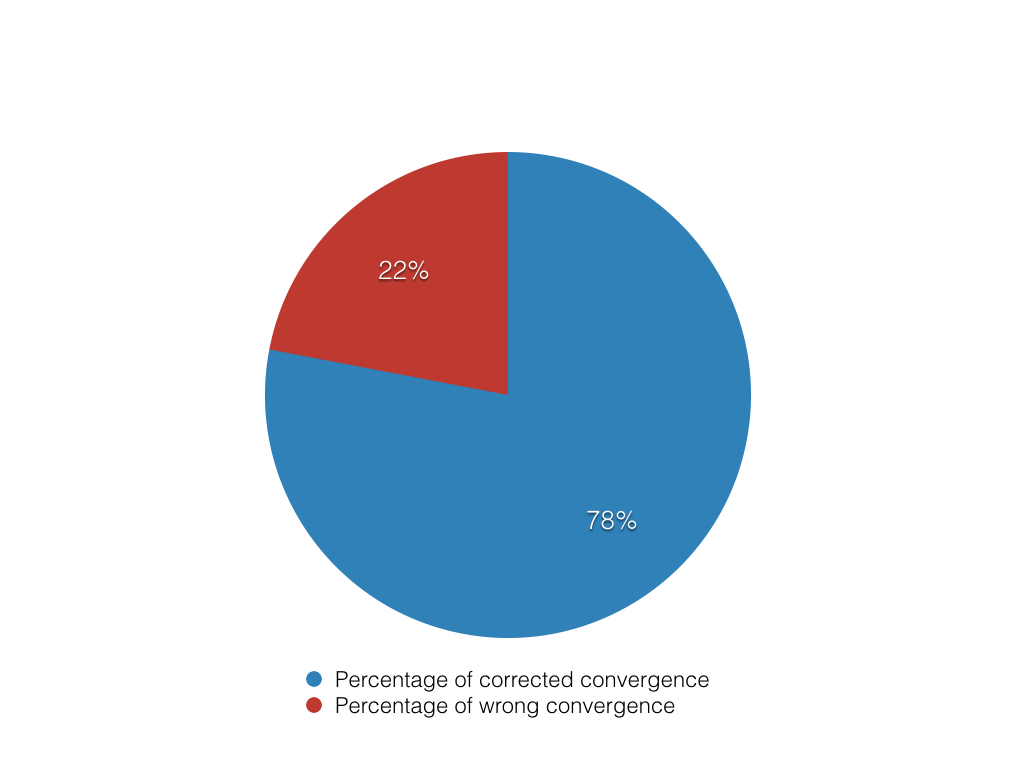
\includegraphics[width=0.5\textwidth]{s2}
		\label{fig:ost12}}
	\caption{Summary results with two memories}
	\label{fg:ost1}
\end{figure}

Looking at the first two pie charts with only two memories stored in Figure \ref{fg:ost1}, it can be seen that the percentage correct using the standard weights and optimized weights is the same at 78\%.\\

\begin{figure}[h]
	\centering
	\subfloat[Subfigure 1 list of figures text][Standard weights]{
		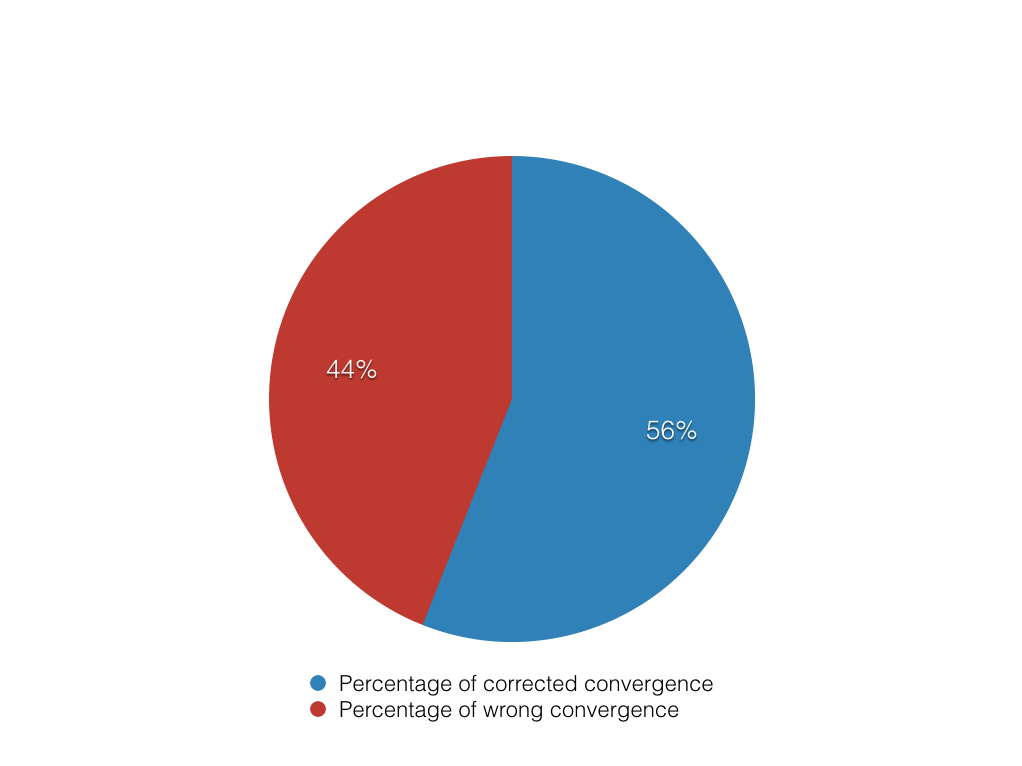
\includegraphics[width=0.5\textwidth]{s3}
		\label{fig:ost21}}
	\subfloat[Subfigure 2 list of figures text][Optimized weights]{
		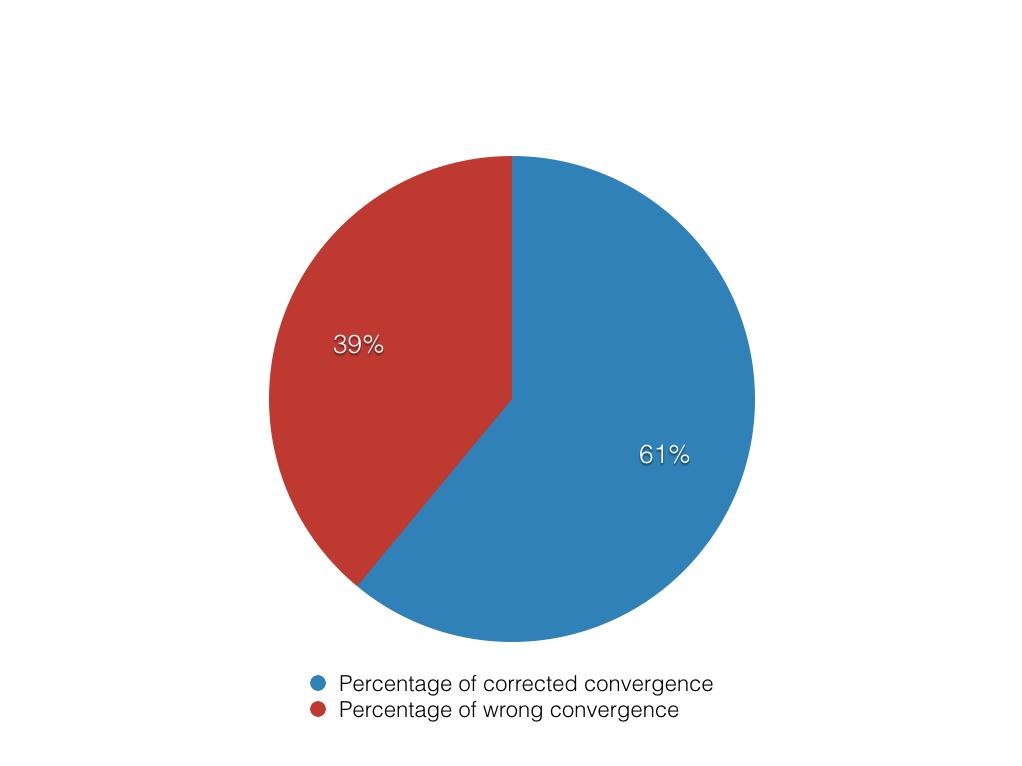
\includegraphics[width=0.5\textwidth]{o3}
		\label{fig:ost22}}
	\caption{Summary results with three memories}
	\label{fg:ost2}
\end{figure}

In Figure \ref{fg:ost2}, when storing only three memories, that percent correct for the standardized weights drops to 56\%, and the percent correct for the optimized weights jumps to 61\%. Thus both percentages have dropped, but it can be seen that the optimized weights is performing slightly better.\\

\begin{figure}[h]
	\centering
	\subfloat[Subfigure 1 list of figures text][Standard weights]{
		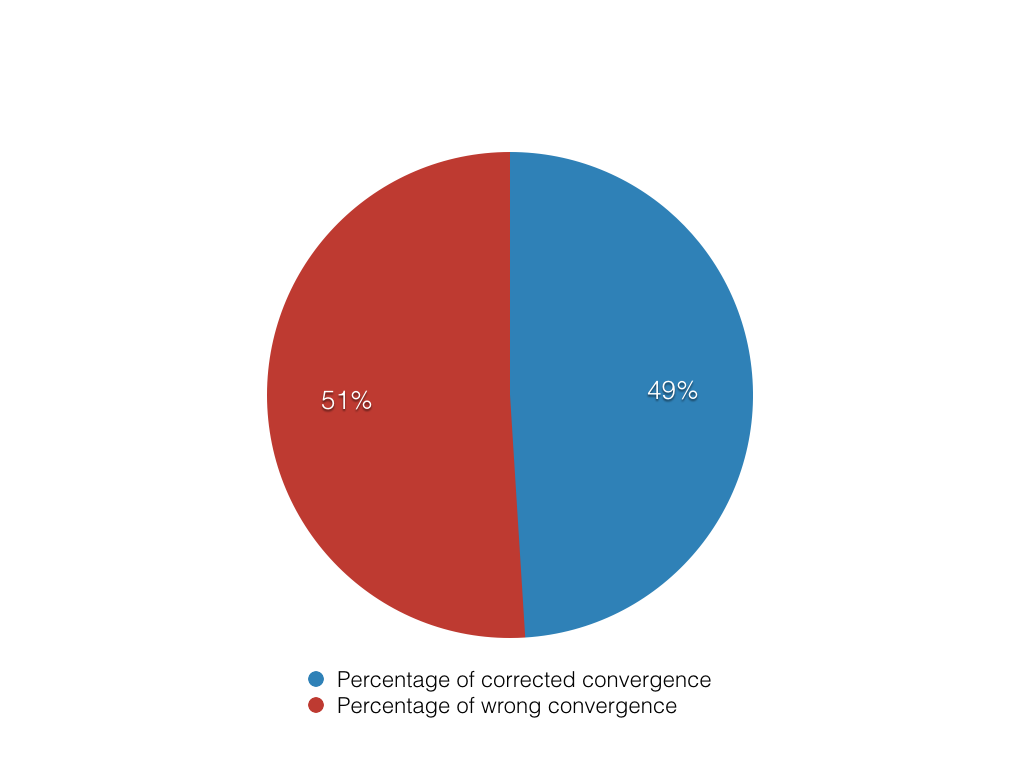
\includegraphics[width=0.5\textwidth]{s5}
		\label{fig:ost31}}
	\subfloat[Subfigure 2 list of figures text][Optimized weights]{
		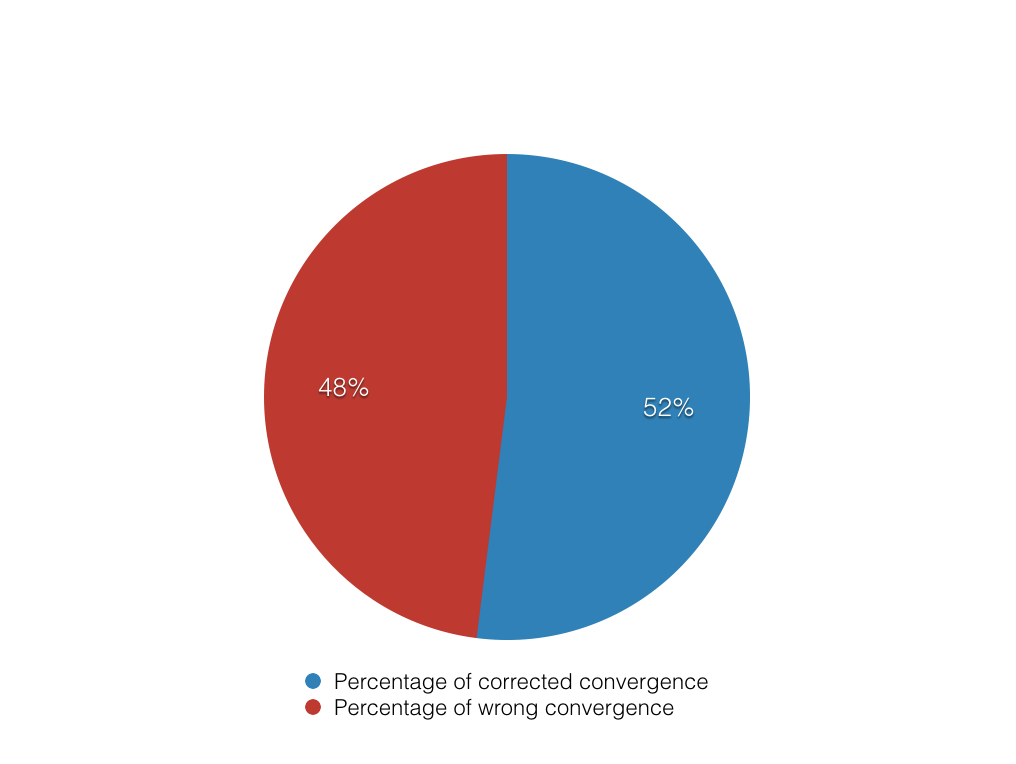
\includegraphics[width=0.5\textwidth]{o5}
		\label{fig:ost32}}
	\caption{Summary results with five memories}
	\label{fg:ost3}
\end{figure}

Looking at Figure \ref{fg:ost3}, with five memories stored, the percent correct for the standard weights drops to 49\% and for the optimized weights drop to 52\%. This is a smaller gap between the performance of the standard vs optimized weights, but the optimized weights are still outdoing the standard weights.\\

\begin{figure}[h]
	\centering
	\subfloat[Subfigure 1 list of figures text][Standard weights]{
		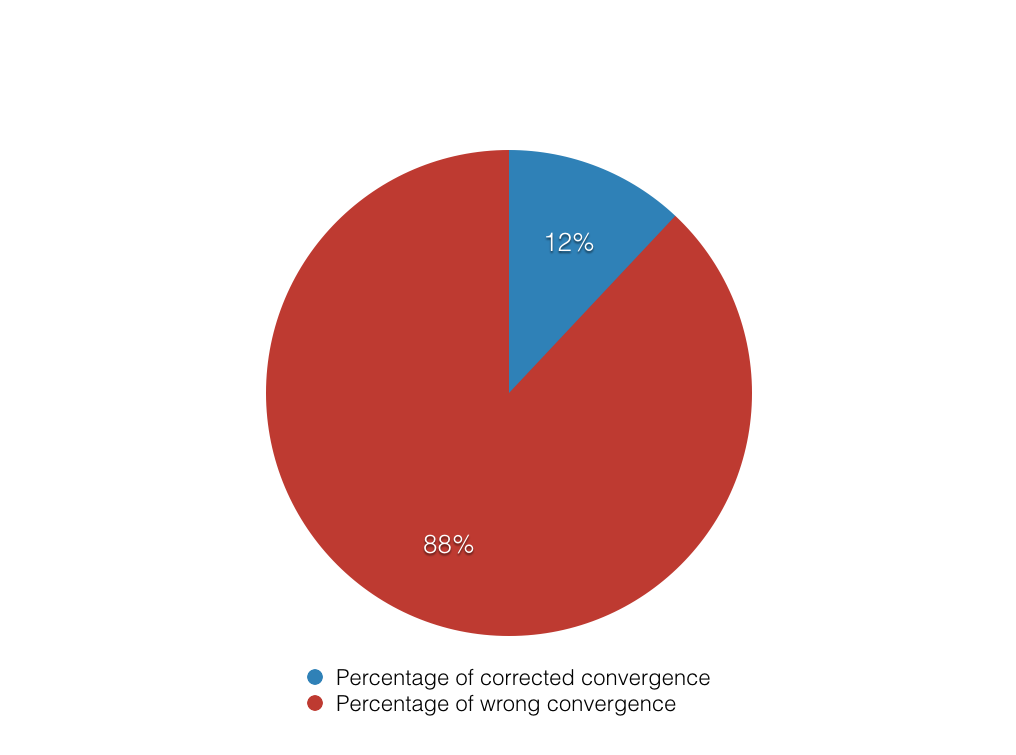
\includegraphics[width=0.5\textwidth]{s9}
		\label{fig:ost41}}
	\subfloat[Subfigure 2 list of figures text][Optimized weights]{
		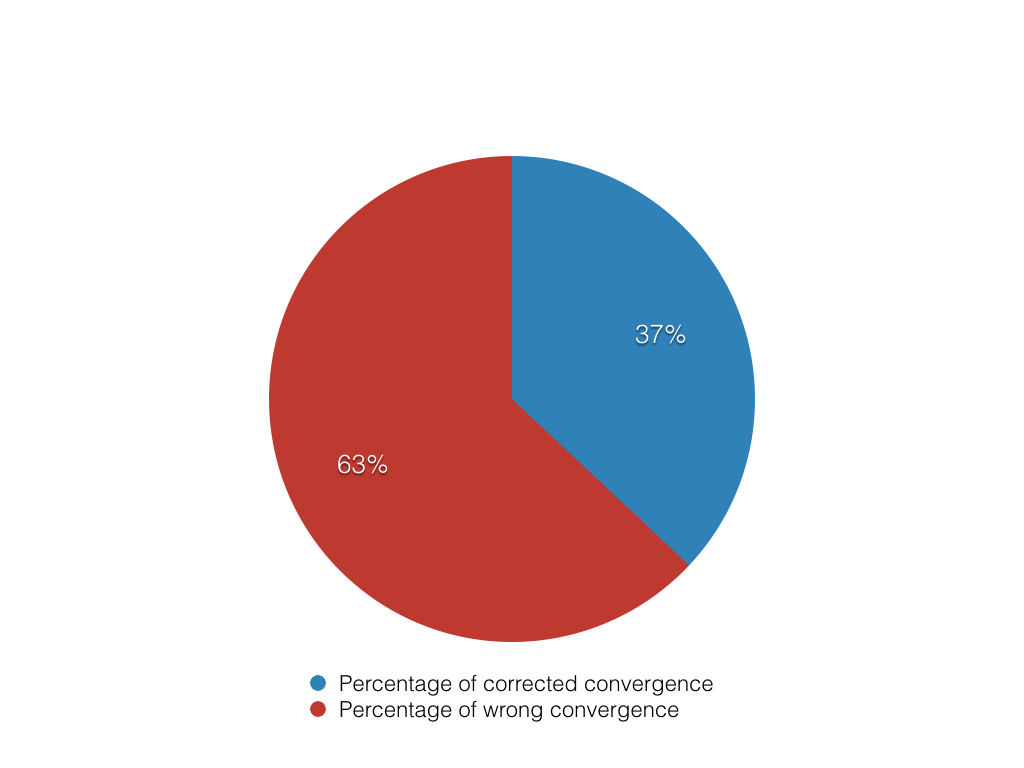
\includegraphics[width=0.5\textwidth]{o9}
		\label{fig:ost42}}
	\caption{Summary results with nine memories}
	\label{fg:ost4}
\end{figure}

In Figure \ref{fg:ost4}, with nine memories stored, the percent correct plummets to 12\% for the standard weights and 36\% for the optimized weights. This is a much more noticeable gap between the performance of the standard and optimized weights.\\

\begin{figure}[h]
	\centering
	\subfloat[Subfigure 1 list of figures text][Standard weights]{
		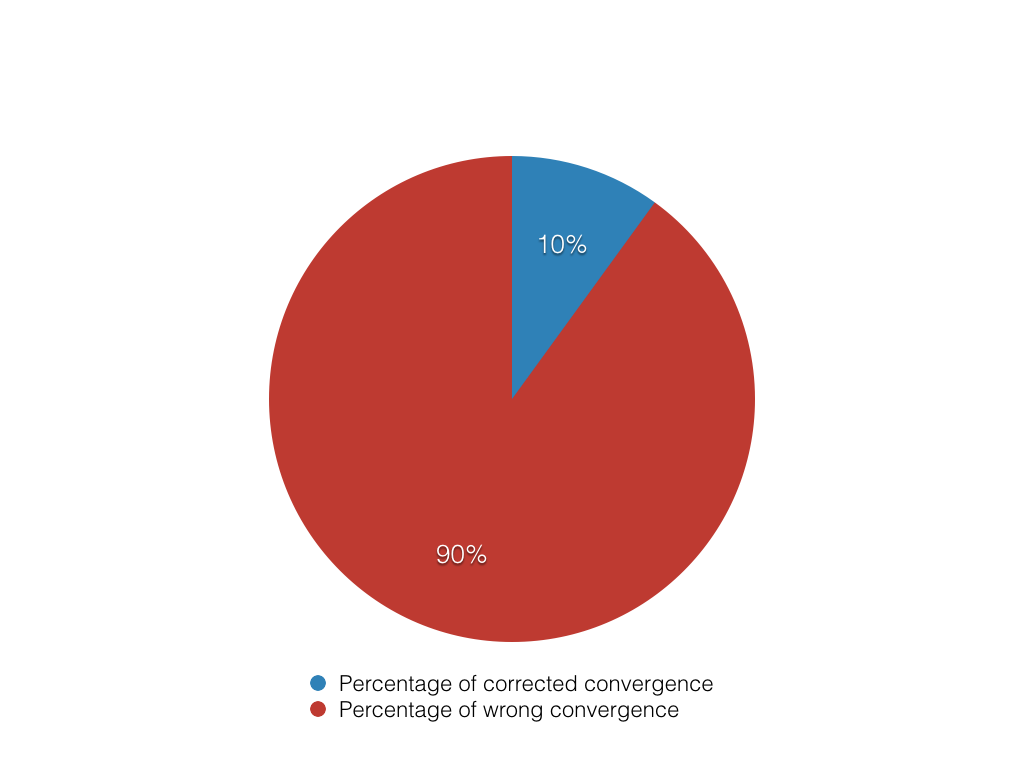
\includegraphics[width=0.5\textwidth]{s10}
		\label{fig:ost51}}
	\subfloat[Subfigure 2 list of figures text][Optimized weights]{
		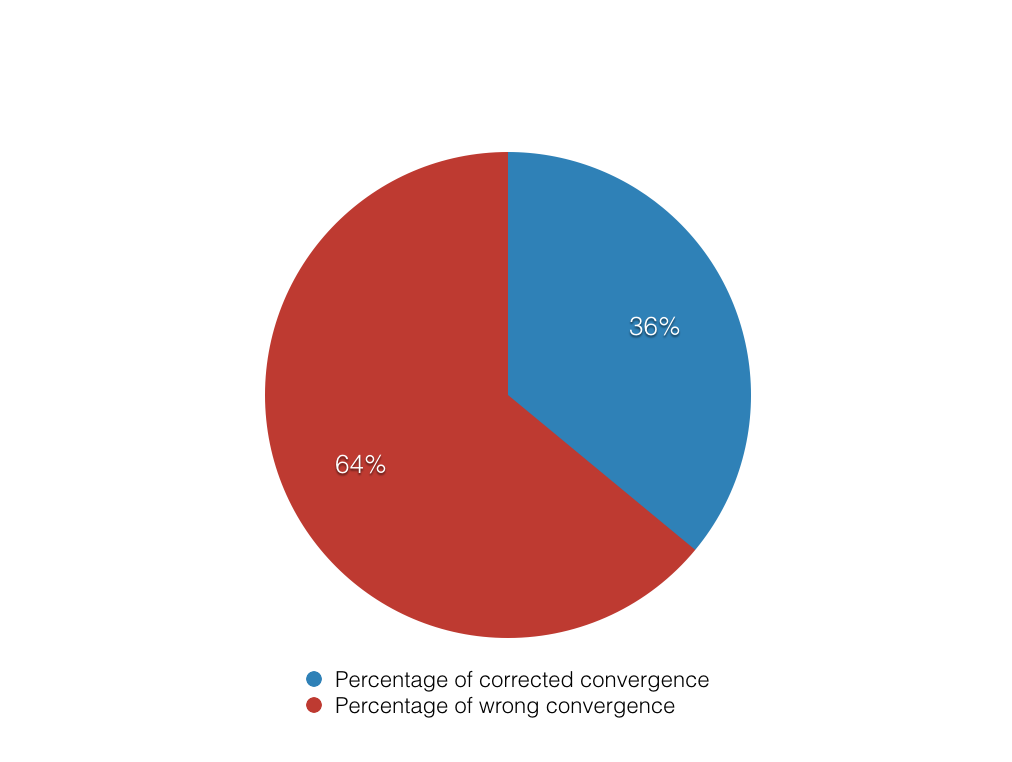
\includegraphics[width=0.5\textwidth]{o10}
		\label{fig:ost52}}
	\caption{Summary results with ten memories}
	\label{fg:ost5}
\end{figure}

Similarly, in Figure \ref{fg:ost5}, with ten memories stored, the percent correct drops to 10\% for the standard weights and remains at 36\% for the optimized weights. This again shows that the optimized weights perform better than the standard weights.\\


